% @Author: AnthonyKenny98
% @Date:   2020-04-06 17:52:43
% @Last Modified by:   AnthonyKenny98
% @Last Modified time: 2020-04-07 12:37:57

\begin{figure}[H]
\begin{centering}
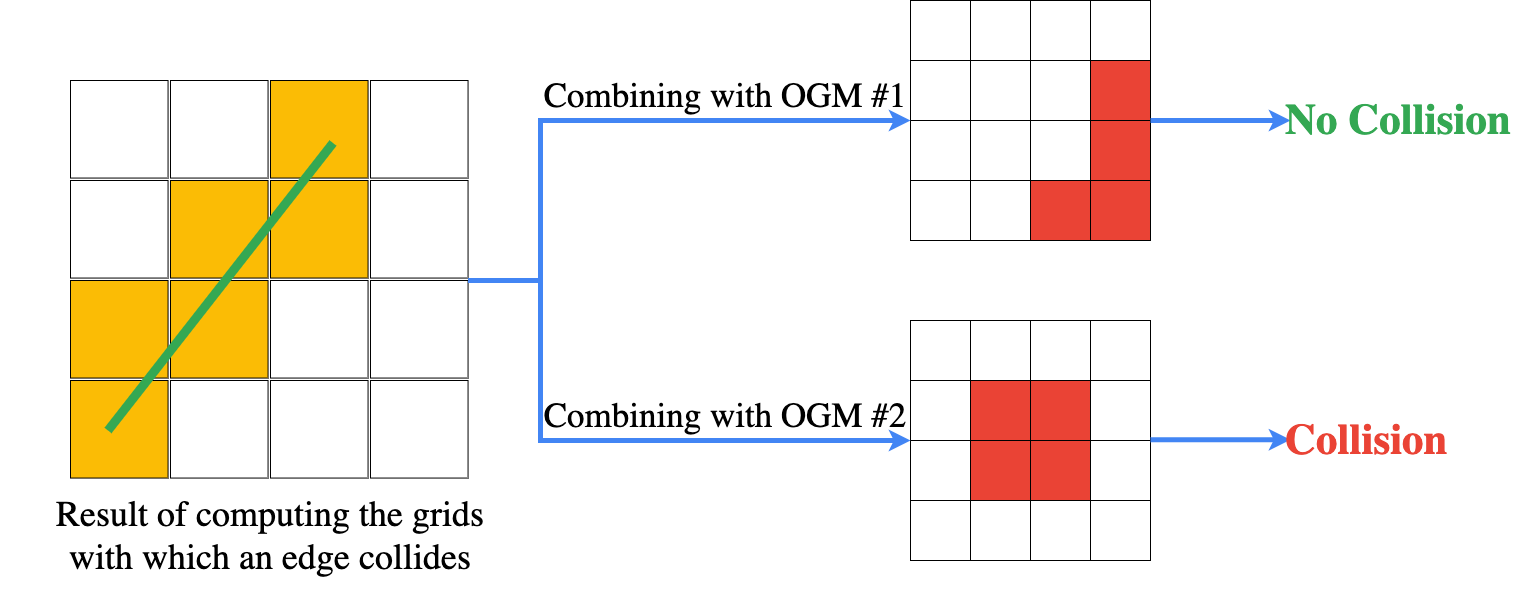
\includegraphics[width=\linewidth]{chapters/chapter3/img/edge_collision_process.png}
\mycaption{Edge Collision Computation Process}{. Most of the computational load is found in determining the grids with which an edge intersects (as seen on the left of the figure). Once these grids have been found, it is very simple (and fast) to lookup if these grids are occupied in the \gls{OGM}}
\label{fig:edge_collision_process}
\end{centering}
\end{figure}